\subsection{Simulations}
When used in the broadest sense of the term, \textbf{modeling} is a central activity in quantitative consulting. As a result, in order to be a successful quantitative consultant, it is important to understand the different types of modeling and models, their commonalities and differences, and relevant and appropriate applications of modeling techniques. At the same time, because of its ubiquity in so many aspects of the quantitative process, the importance of modeling is often overlooked and taken for granted, since it underlies, and is incorporated into, so many other techniques. \textbf{If you are a quantitative consultant you are, by necessity, a modeler}. Consequently, having a strong general understanding of what modeling is (as distinct from particular modeling techniques) and understanding how to construct models in a more general sense, will facilitate many consulting endeavours.
\newl \textbf{Analogical reasoning} is the act of reasoning from one specific occurrence to another specific occurrence, on the basis of similarity. For example, \begin{quote}[HAND:FINGERS, FOOT: ---].\end{quote} A major benefit of this type of reasoning is that it can reveal new aspects or relationships between objects that have not previously been considered. Clearly, the choice of objects used in an analogy is important: \begin{quote} [HAND:FINGERS, ORANGE: ---] \end{quote}
likely yields little useful insight, but 
\begin{quote}[HAND:FINGERS, PLANT STEM: ---] \end{quote}
might be more interesting (see Figure~\ref{simfig:1}). Analogical reasoning is viewed by some as a primary \textbf{cognitive strategy}, underlying much of human cognition \cite{SIM_HGK,SIM_H,SIM_C}.
\begin{figure}[!t]
	\centering
		\includegraphics[width=0.50\textwidth]{images/SIM/analogy_diagram.pdf}
	\caption[\small Example of analogical reasoning]{\small Can you draw an analogy between the top row of shapes and the bottom row of shapes? What should the shape and colour of the final figure in the bottom row be?}
	\label{simfig:1}\hrule
\end{figure}
\newl Keeping this context in mind, a model is simply an independent entity, or structure, that has useful similarities to another structure of interest, and which allows for analogical reasoning. This structure of interest is referred to as the target of the model. We can carry out inductive or deductive reasoning on the model and then, via analogical reasoning, transfer our insights about the model over to the target, and in this way learn something about the target. The target structure might be a single object or a system of objects, or a process being carried out by this system of objects.

Our ability to create a model with \textit{useful similarities} to the target system, and then learn about our chosen target system using this model, can be extremely powerful. For example, we can make a very small model of something that is, in reality, very large or very distant -- for example, a small scale model of the solar system, made out of wire and styrofoam -- and use this small simple model to come up with accurate predictions about this large and distant system. \par The solar system model example also showcases the importance of understanding \textbf{which parts of the model are usefully similar to the target system} in the context of our intended use of the model. If we try to use our simple solar system model to draw conclusions relating to the relative densities of planets in the solar system, we will be disappointed.
\newl Although there are many different types of models, which we will further discussed later, in general we can say that models have two main functions: \textbf{explanation} and \textbf{prediction}. 
\begin{itemize}[noitemsep]
\item In some cases, we might have a system whose behaviour we do not fully understand and cannot explain. Models can help us  increase our understanding of the mechanisms underlying the behaviours or properties of interest. 
\item In other cases, regardless of how a type of system is generating a particular behaviour, or came to have a certain property, our interest is not in understanding how this came to be, but rather in predicting the presence (or absence) of that behaviour or property in another system of the same type.
\end{itemize}
Modelers often try to create \textbf{taxonomies} or categorisations of models. These efforts have arguably not been that successful from a conceptually rigorous point of view but, pragmatically, it is still useful to consider the types of models that people commonly talk about (see \cite{SIM_Y} for a useful review and discussion of a variety model and simulation types).
\begin{center}\rule{0.5\linewidth}{.4pt}\end{center}
\textbf{IMPORTANT NOTE:} it has been our experienced that clients usually take a dim view of simulations, as though they are less `valid' or `real` than other quantitative approaches. The reasons for this are varied, and perhaps not entirely unfounded as simulations can easily be used in the wrong way or with the wrong endgame in mind. \par We discuss, in the following pages, a number of strategies to help consultants provide sound simulation solutions for their client. 
\subsubsection{Static Models}
Central to the idea of simulations is the notion of a \textbf{model}. There are numerous modeling strategies -- ultimately, however, all models are used with the goal of helping the modeler better understand a \textbf{system} (a term that we will use in an axiomatic fashion). 
\paragraph{Conceptual Models}

A conceptual model is an \textbf{abstraction of a real world system} or process that defines which elements of that system or process are of interest in the current context, and how these elements and their relationships will be defined for the purposes of \textbf{drawing conclusions} about the behaviours or properties of the system. Arguably, before any other type of model can be generated, a conceptual model must first be created, either implicitly or explicitly. 

\textbf{Explicit conceptual models} may take the form of diagrams or formalised descriptions of the system. Conceptual models may then be implemented as other types of models (e.g. mathematical, simulation). 

{Implicit conceptual models} are often linked with gaps in the understanding of a system -- assumptions that go unchallenged and unstated are often less clear and obvious than is originally believed. An engineer may, for instance, state to a consultant that the probability of a certain component failing by time $t$ is 0 without feeling the need to specify that, in the jargon of the discipline, this really means that $$P(\textrm{failure by time }t>T)>\varepsilon>0,\quad \mbox{for a sufficiently large } T \mbox{ and a sufficiently small }\varepsilon;$$ the consultant, not knowing the conventions of the field, might understand this to mean that  $$P(\textrm{failure by time }t)=0\quad \mbox{for all } t,$$ and the mistake can propagate through the simulation, potentially making the simulation useless in practice.   

\paragraph{Mathematical Models}

A mathematical model uses mathematical expressions to \textbf{support reasoning} about a real world system. Relationships between objects in the system, or their properties, are represented by mathematical relationships between variables. If the relationships within the mathematical model are \textbf{sufficiently similar} to relationships between objects in the system of interest, then carrying out mathematical methods (truth preserving manipulations) on the model should result in new true conclusions about the system. 

Note that arguments represented by symbolic logic also fall under this category. As a result, it could readily be said that all models implemented on computers are a type of mathematical model. That being said, the expression `mathematical model' typically refers to models that are not necessarily implemented on computers, and which consist of systems of mathematical equations.
\newl Although mathematical models may represent processes and dynamic elements of systems by including time and space as variables, the models themselves are \textbf{static}, in the sense that they do not change over time in a manner that is similar to the ways in which the target system itself changes over time. Mathematical models may still be implemented on computers and methods for \textbf{solving the systems of equations} in these models (e.g. symbolic manipulations, numerical analysis) may be carried out using computer algorithms, however, the fact that this work is carried out on a computer, and the fact that simulations are also carried out on a computer, does not mean that finding solutions to equations using programmatic strategies is the same as carrying out simulations, in the way that the term `simulation' is typically used. Simulations will be further discussed below.

\paragraph{Statistical Models}

Conceptually speaking, statistics represents the world in terms of \textbf{populations} and \textbf{processes}. These populations and processes then have certain properties, which can be represented themselves using mathematical expressions. Statistical models could thus be described as mathematical models motivated by a certain (statistical) conceptualisation of real world processes. 


\paragraph{To-Scale Physical Models}

A to-scale physical model is a model that is constructed from \textbf{physical materials}, which are shaped and positioned in such a way as to accurately represent the physical layout and positions of elements of the target system, as well as their size, relative to each other (see Figure~\ref{simfig:2} for an example of an architectural model).

\begin{figure}[!t]
	\centering
		\includegraphics[width=0.68\textwidth]{images/SIM/Architectural_model_condo_interior.jpg}
	\caption[\small A to-scale architectural model]{\small To-scale architectural model of the interior of an office building \cite{SIM_TSAM}.}
	\label{simfig:2}\hrule
\end{figure}
\afterpage{\FloatBarrier}


\paragraph{Data Models}

A data model is a conceptual model used to design the structure of data storage. Since data itself represents facts about a system, it is appropriate to first conceptually model the properties and relationships that exist within the system, and which are represented by the data, and then use this conceptual model to create a data storage structure that can be used to efficiently \textbf{hold}, \textbf{extract}, \textbf{edit} and \textbf{add} to the stored data (see Figure~\ref{simfig:3} for an example).

\begin{figure}[!t]
	\centering
		\includegraphics[width=0.96\textwidth]{images/SIM/data-systemmodel.pdf}
	\caption[\small An example of a data model]{\small A preliminary data model of a restaurant reservation system, which can be used to help design an efficient data storage structure, as well as develop data analysis strategies.}
	\label{simfig:3}\hrule
\end{figure}


\subsubsection{Dynamic Models}

In some situations, only the static aspects of a system are interesting, or the system itself is mostly static. For example, if we build a physical model of a house, we expect both the house and the model to be \textbf{relatively unchanging} -- the measurements of the rooms and the furniture in the house will not change from minute to minute (although they could change over years due to remodeling, or drastically if the house is sold to new owners with a different sense of aesthetics), and the model will not need to change either. We can then use the model to reason about the house: 
\begin{itemize}[noitemsep]
\item if the model couch fits against this wall in the model house, we can reason that the real couch will fit in the real house;
\item if eight model chairs cannot simultaneously be placed around the model kitchen table, than eight real chairs cannot be simultaneously be placed around the real kitchen table, etc.
\end{itemize}
Other systems, however, are more active, or \textbf{dynamic}, with processes taking place within the system. When modeling these dynamic system elements, we often talk about \textbf{simulation models} or simply \textbf{simulations}. Although the term `simulation' is not precisely defined, it typically indicates that a model is intended to \textbf{reflect the behaviour of the target system} -- its processes -- over time, and also that the \textbf{model itself will independently change over time}, when it is run. The goal is to construct the simulation in such a way that it will change over time in ways that are similar to the manner in which the system itself changes over time. As a result we can use the simulation to predict past, current, and future behaviours of the system. Historically speaking, simulations have often modeled individual object-level properties and behaviours, as well as the mechanisms underlying relevant behaviours, rather than group level properties or system outputs, but this does not have to be the case.
\newpage\noindent
\paragraph{Modeling Time and Movement}

How do we incorporate time and movement into a model? To return to our styrofoam and wires model of the solar system, if we set up our model such that when we turn a crank the planets and moons realistically move around a light bulb in the centre of the model (representing the sun), then we have a dynamic model, or simulation of the solar system. We can simulate what will happen within the actual solar system over time. \par As another example, if we wish to know how emergency responders might behave in different plane crash scenarios, we could set up a number of simulated crash scenarios, with a life-size model of a crashed plane, and actors behaving as injured people might. We can then have the emergency responders try out (i.e. simulate) different approaches and strategies to dealing with plane crashes.
\newl The advent of computers greatly facilitated the construction and possible uses of simulations, because it made it possible to simulate dynamic systems \textbf{virtually} instead of having to create a dynamic physical model of the system, whose elements could be represented as data structures (and variables within these structures) within computer programs. The physical interactions between these system elements could then, in turn, be represented by logical rules and mathematical equations operating over these data structures.

These logical rules and mathematical equations pushed computer simulations closer to the domain of mathematical models, relative to physically constructed models. At the same time, computer simulations retained the strategy used by these physical models of determining what would happen to the system by moving the model through its expected behaviours step-by-step, over time. Rather than mechanically moving the model (or using people and other elements in this capacity) computer models rely on the computer processor to run the program that represents the system, and essentially `move' (in an electronic sense) the model based on the behaviours the model implements. As discussed earlier, this is a different technique than the one used by mathematical models implemented on computers.

\subsubsection{Uses, Data, and Contrast with Mathematical Modeling}

Simulations are typically used to 
\begin{itemize}[noitemsep]
\item better understand actual real-world phenomena and systems, and 
\item explore phenomena that don't currently exist but which could exist hypothetically. 
\end{itemize}
Simulations can allow us to both \textbf{predict} what our target system will do under particular circumstances, but also \textbf{explain} why a system behaves the way it does. However, given that we build simulations using only what is already known (or possibly suspected) to be either currently the case about the system, or at least plausible within the conceptual phase space in which the system resides, you may wonder how a simulation could possibly tell us anything new about the system, and thus, why we would ever bother running simulations. \par Humans thinking is typically unable to capture all the possible interactions between a system's various parts, and how these parts influence each other in particular circumstances; \textbf{merely} thinking through the behaviours of a system which is even slightly complicated is likely lead us to miss implications, and, as a result, \textbf{incorrectly predict or explain} the system's behaviour. If, instead, we introduce what we do know into the simulation and allow it to behave based on these rules, behaviours that we would not easily have anticipated can emerge from the process.
\newpage\noindent Consequently, the notion of \textbf{emergence} is crucial in simulations. We can say that simulation behaviours emerge when they are not programmed in the simulation directly, but rather occur as the result of interactions between model components that are themselves programmed into the simulation directly. \par The emergent behaviours may occur at different \textbf{levels of granularity} of the system. For example, if we create a simulation of people in a city, we might see emergent behaviour with respect to which people most frequently interact with which other people, and we might also see emergent behaviour at the population level, where the average number of people in a given location is equal to a particular value over time.

We can see from this example how emergence allows us both to predict and to explain elements of a system that were not previously amenable to such efforts. We can predict average numbers of people in a particular location, if this information is not available from another source; if it is, we can still use the simulation to explain the origins and underpinnings of this number, by referring to the more granular system components whose interactions lead to the value.
\newl \textbf{IMPORTANT NOTE:} `emergence' is a concept that has crossed-over into a large number of areas of human endeavour. Don't be surprised to hear clients talk about ``emergent phenomena'' in contexts where you would not normally expect to hear it. It is quite conceivable that they have a very thorough understanding of what emergence means and what it entails -- don't make  the classic quantitative consulting mistake of assuming that clients do not understand technical concepts ... you never know what their background and interests are -- but, together with terms like `synergy' or `big data', it seems to have entered the business lexicon as a trendy but ultimately meaningless term. Be sure to clarify the situation at an early stage (by definining concepts in the proposal, say) in order to avoid the confusion and headaches that can result when deliverables are handed off. 
\begin{center}\rule{0.5\linewidth}{.4pt}\end{center}
\paragraph{Simulations and Data}

All modeling activities rely on the modeler having \textbf{accurate} and \textbf{relevant} information or data about the target system, which allows for the construction of a model with useful similarities to the target system, which is basically a data collection/information gathering problem. But even then,  simulations have a particular relationship with data:
\begin{itemize}[noitemsep]
\item first and foremost, data is needed in order to properly set simulation parameters -- the initial simulation settings that determine how the simulation will run in a particular instance; in the absence of this type of information, although the simulation may generate outputs that could, in principle, have some relevance to the target system in some circumstances, the simulation behaviour is unlikely (or at least, should not be expected) to overlap with target system behaviours of interest within the specific context in which the simulation was generated;
\item secondly, simulations have the capacity to generate large amounts of data about the behaviour of the simulation, and by extension, the target system. This data, sometimes referred to as `synthetic data' or `simulated data', can be uses as a stand-in for actual data about the system, just as the model is being used as a stand-in for the target system.
\end{itemize}
When very little is know about reasonable parameters values, a preliminary simulation might first be required in order to produce data which could then be used to set simulation parameters, which, in turn, could be used to produce data for analysis. It is not too difficult to conceive of multiple links being added to this chain; our advice is to keep the number of such links to a minimum (preferably zero) -- in light of the point made in the first item above, it might be preferable to garner information about parameters from \textbf{first principles} (or other models).  
\paragraph{Simulations vs. Mathematical Models}
The procedural element of computer models, whereby the behaviour of the target system must be, in a sense, mechanically replicated by the data structures and procedures of the computer program, distinguishes \textbf{computer simulations} from mathematical models, which, rather than modeling the temporal, dynamic components of systems by incorporating a temporal, dynamic component directly into the model, instead represent them as variables in mathematical equations that represent components and behaviours of the system.

On this front, the advantage of mathematical models is that \textbf{deductive reasoning} (or first principles reasoning) can, in theory, be used to determine the target system behaviour, rather than have to resort to `running' the model over a range of starting conditions. This is appealing, as mathematical strategies can allow for more definitive and general statements about the system (e.g. ``The system will never do the following''; ``The system will always do the following'', etc.); these types of  statements are typically outside the reach of even the most advanced  mechanical or programmatic simulations. In practice, however, the underlying complexity of such models limit the usefulness of this approach in most scenarios.
\begin{center}\rule{0.5\linewidth}{.4pt}\end{center}
Consider, for example, the \textbf{$n-$body problem} ($n$BP) of classical mechanics, which consists in predicting the individual trajectories of $n$ celestial bodies bound by gravitational attraction. \par Using Newtonian meachanics, the trajectories can be deduced to follow the paths described by the following system of differential equations: 
\begin{align*}
m_1\frac{\textrm{d}^2\mathbf{q}_1}{\textrm{d}t^2}&=\sum_{j=2}^n\frac{Gm_1m_j(\mathbf{q}_j-\mathbf{q}_1)}{\|\mathbf{q}_j-\mathbf{q}_1\|^3} \\
m_2\frac{\textrm{d}^2\mathbf{q}_2}{\textrm{d}t^2}&=\sum_{j\neq 2}^n\frac{Gm_2m_j(\mathbf{q}_j-\mathbf{q}_2)}{\|\mathbf{q}_j-\mathbf{q}_2\|^3} \\
& \vdots \\ 
m_n\frac{\textrm{d}^2\mathbf{q}_n}{\textrm{d}t^2}&=\sum_{j= 1}^{n-1}\frac{Gm_nm_j(\mathbf{q}_j-\mathbf{q}_n)}{\|\mathbf{q}_j-\mathbf{q}_n\|^3},
\end{align*}
where $m_i$ and $\mathbf{q}_i(t)$ are, respectively, the mass and the trajectory of the $i^{\textrm{th}}$ celestial body in 3-space, and $G$ is Newton's constant. These equations describe, in principle,  the behaviour of stars in a globular cluster, say, or of the Earth-Sun or the Earth-Moon system. They cannot provide a \textbf{complete} description as the range of gravitational attraction is infinite -- every `object' in the Universe influences every `other' object to some extent, no matter how distant (see the precession of Mercury, for instance), and other forces may also act on the bodies (but at large distances, the force due to gravity overwhelms the other 3 forces), but, for most practical applications (if one can consider astronomy a practical discipline), they are more than sufficient, as long as we are willing to ignore relativistic effects.  
\newpage\noindent What do the solutions look like? A typical mathematical approach would be to try to solve the 2BP, and to see if the solution can be generalised to more complex cases. \par The \textbf{two-body problem} has an exact solution. The centre of mass of the two bodies is the vector $$\mathbf{x}(t)=\frac{m_1\mathbf{q}_1(t)+m_2\mathbf{q}_2(t)}{m_1+m_2}.$$ In the centre-of-mass frame (that is, in the frame that moves along with the centre of mass), it can be shown, using physical conservation laws, that the trajectories of the two bodies are co-planar and `orbit' the system's barycentre, with an angle $\theta_i(t)$ which depends on the reduced mass of the system $m_*=\frac{m_1m_2}{m_1+m_2}$ and on the effective potential $U(r(t),\ell,m_*)$, where $r(t)=\|\mathbf{q}_2-\mathbf{q}_1\|$ and $\ell$ is the system's angular momentum. \par Various combinations of parameters lead to various orbits; if the effective potential admits a local minimum, for instance, the orbits will oscillate around the barycentre (elliptic or precessing elliptic paths, in each Sun-planet system); if the effective potential does not admit a minimum, then the orbits may escape to infinity (hyperbolic or parabolic paths, such as in some Sun-comet systems).\newl  Under some restrictions on the masses and momenta of the bodies, the $n$BP can be shown to have closed-form solutions or theoretically understood approximate solutions 
\begin{figure}[!t]
\centering
\begin{subfigure}[m]{0.3\textwidth}
\includegraphics[width=\textwidth]{images/SIM/nbp1.png}
\caption{\small Planetary 3BP}
\end{subfigure}\quad
\begin{subfigure}[m]{0.3\textwidth}
\includegraphics[width=\textwidth]{images/SIM/nbp2.png}
\caption{\small 4BP pairs of bodies orbiting each other}
\end{subfigure}\quad 
\begin{subfigure}[m]{0.3\textwidth}
\includegraphics[width=\textwidth]{images/SIM/nbp3.png}
\caption{\small 3-body choreography}
\end{subfigure}
\caption[\small Possible solutions of the $n-$body problem]{\small Possible solutions of the $n-$body problem, based on \cite{SIM_WUM}.}\label{fig:nbp}\hrule\end{figure}(see \cite{SIM_NBP} for a list, and Figure~\ref{fig:nbp} for some illustrations), including: 
\begin{itemize}[noitemsep]
\item \textbf{Euler's Problem of Two-Fixed Centres} allows for colinear motion in systems where two of the three masses are comparable and fixed;
\item the \textbf{restricted} 3BP shows the existence of 5 fixed configurations (involving the \textbf{Lagrangian points}) which rotate around the system's  barycentre in cases where one of the masses is negligible, such as is the case in the Sun-Jupiter-Trojans systems (there are two);
\item the \textbf{planetary} $n$BP admits quasi-periodic solutions in systems where one of the masses is significantly larger than the other $n-1$ masses, which shows that planets in stable, planar, and nearly circular orbits around a star \textit{can} transition to chaotic orbits, but that these orbits would be bounded by quasiperiodic tori and so would preserve some regularity, and
\item \textbf{$n-$}body choreography in which all the masses move on the same manifold, without collisions. 
\end{itemize}  
The \textbf{general} $n-$body problem can be solved analytically using Taylor Series (known as Sundman's series), but the series converge so slowly as to be of no practical use for astronomical results (which would require at least $10^{8000000}$ terms in the 3BP case, well beyond even what modern computers can produce \cite{SIM_B}. A whimsical take on the effects of such unpredictable behaviour is offered in Liu Cixin's  \textit{The Three-Body Problem} \cite{SIM_LC}. 
\begin{center}\rule{0.5\linewidth}{.4pt}\end{center}
By contrast, to draw conclusions from a simulation you must set certain initial conditions and then run the simulation and examine the resulting output. Each simulation run represents only one specific instance in the model space. As a result, it can be difficult, if not downright impossible, to draw general conclusions from the results of one or even multiple simulation runs (to say nothing of exploring the outcome of using different parameter values). \par This has lead to criticism over the use of simulations in some milieus, on the basis that simulations should \textbf{never} be used if mathematical models can be used instead.\newl  However, the $n$BP illustrates why taking this hardline position may be inadvisable; clearly, there are   circumstances in which it is difficult to create solvable (actionable) mathematical models of a system that represents the target system in ways sufficiently similar to the system in relevant respects in order to for salient and accurate conclusions to be drawn about that system, in which case a simulation might provide greater insight. It is also possible to create hybrids of mathematical and simulation models to allow for increased insight into system behaviours.
\begin{center}\rule{0.5\linewidth}{.4pt}\end{center}
If $n$ is relatively small, the $n$BP trajectories can be approximated to a high-level of accuracy by using numerical methods to solve the corresponding system of differential equations (see \cite{SIM_NBODY1} for an example of planetary system formation). For astronomical bodies that avoid collisions (or near encounters), there are two main technical issues:
\begin{itemize}[noitemsep]
\item the first one is that the $n$BP problem is \textbf{chaotic} for $n>2$, so that small errors (such as are generated by truncating initial conditions or intermediate calculations) may lead to simulated solutions that are wildly divergent from the true paths; \item astronomical simulations typically run over million of years, leading to an accumulation of integration errors; this is problematic as the approximate solutions are only mathematical objects, whereas the actual bodies they represent have to satisfy physical laws (including the various conservation laws); this can be tackled by using analytical methods such as the \textbf{variational principle} and \textbf{perturbation theory} to  produce trajectory manifolds on which to `project' the integrated approximations.  
\end{itemize}
For many bodies, the time complexity is related to the square of the number of bodies (more on this later), which can make the direct simulation unpractical. In that case, useful simulations must approximate the essential character of the actual trajectories  while reducing the computational complexity. There are many dedicated methods to achieve this goal (including so-called \textbf{tree code} and \textbf{particle mesh} methods) \cite{SIM_NBP}. \newpage\noindent While these particular issues may not apply to general simulations, the interplay of valid approximation and computational feasibility lies at the core of successful simulations.  
\begin{figure}[!t]
\centering
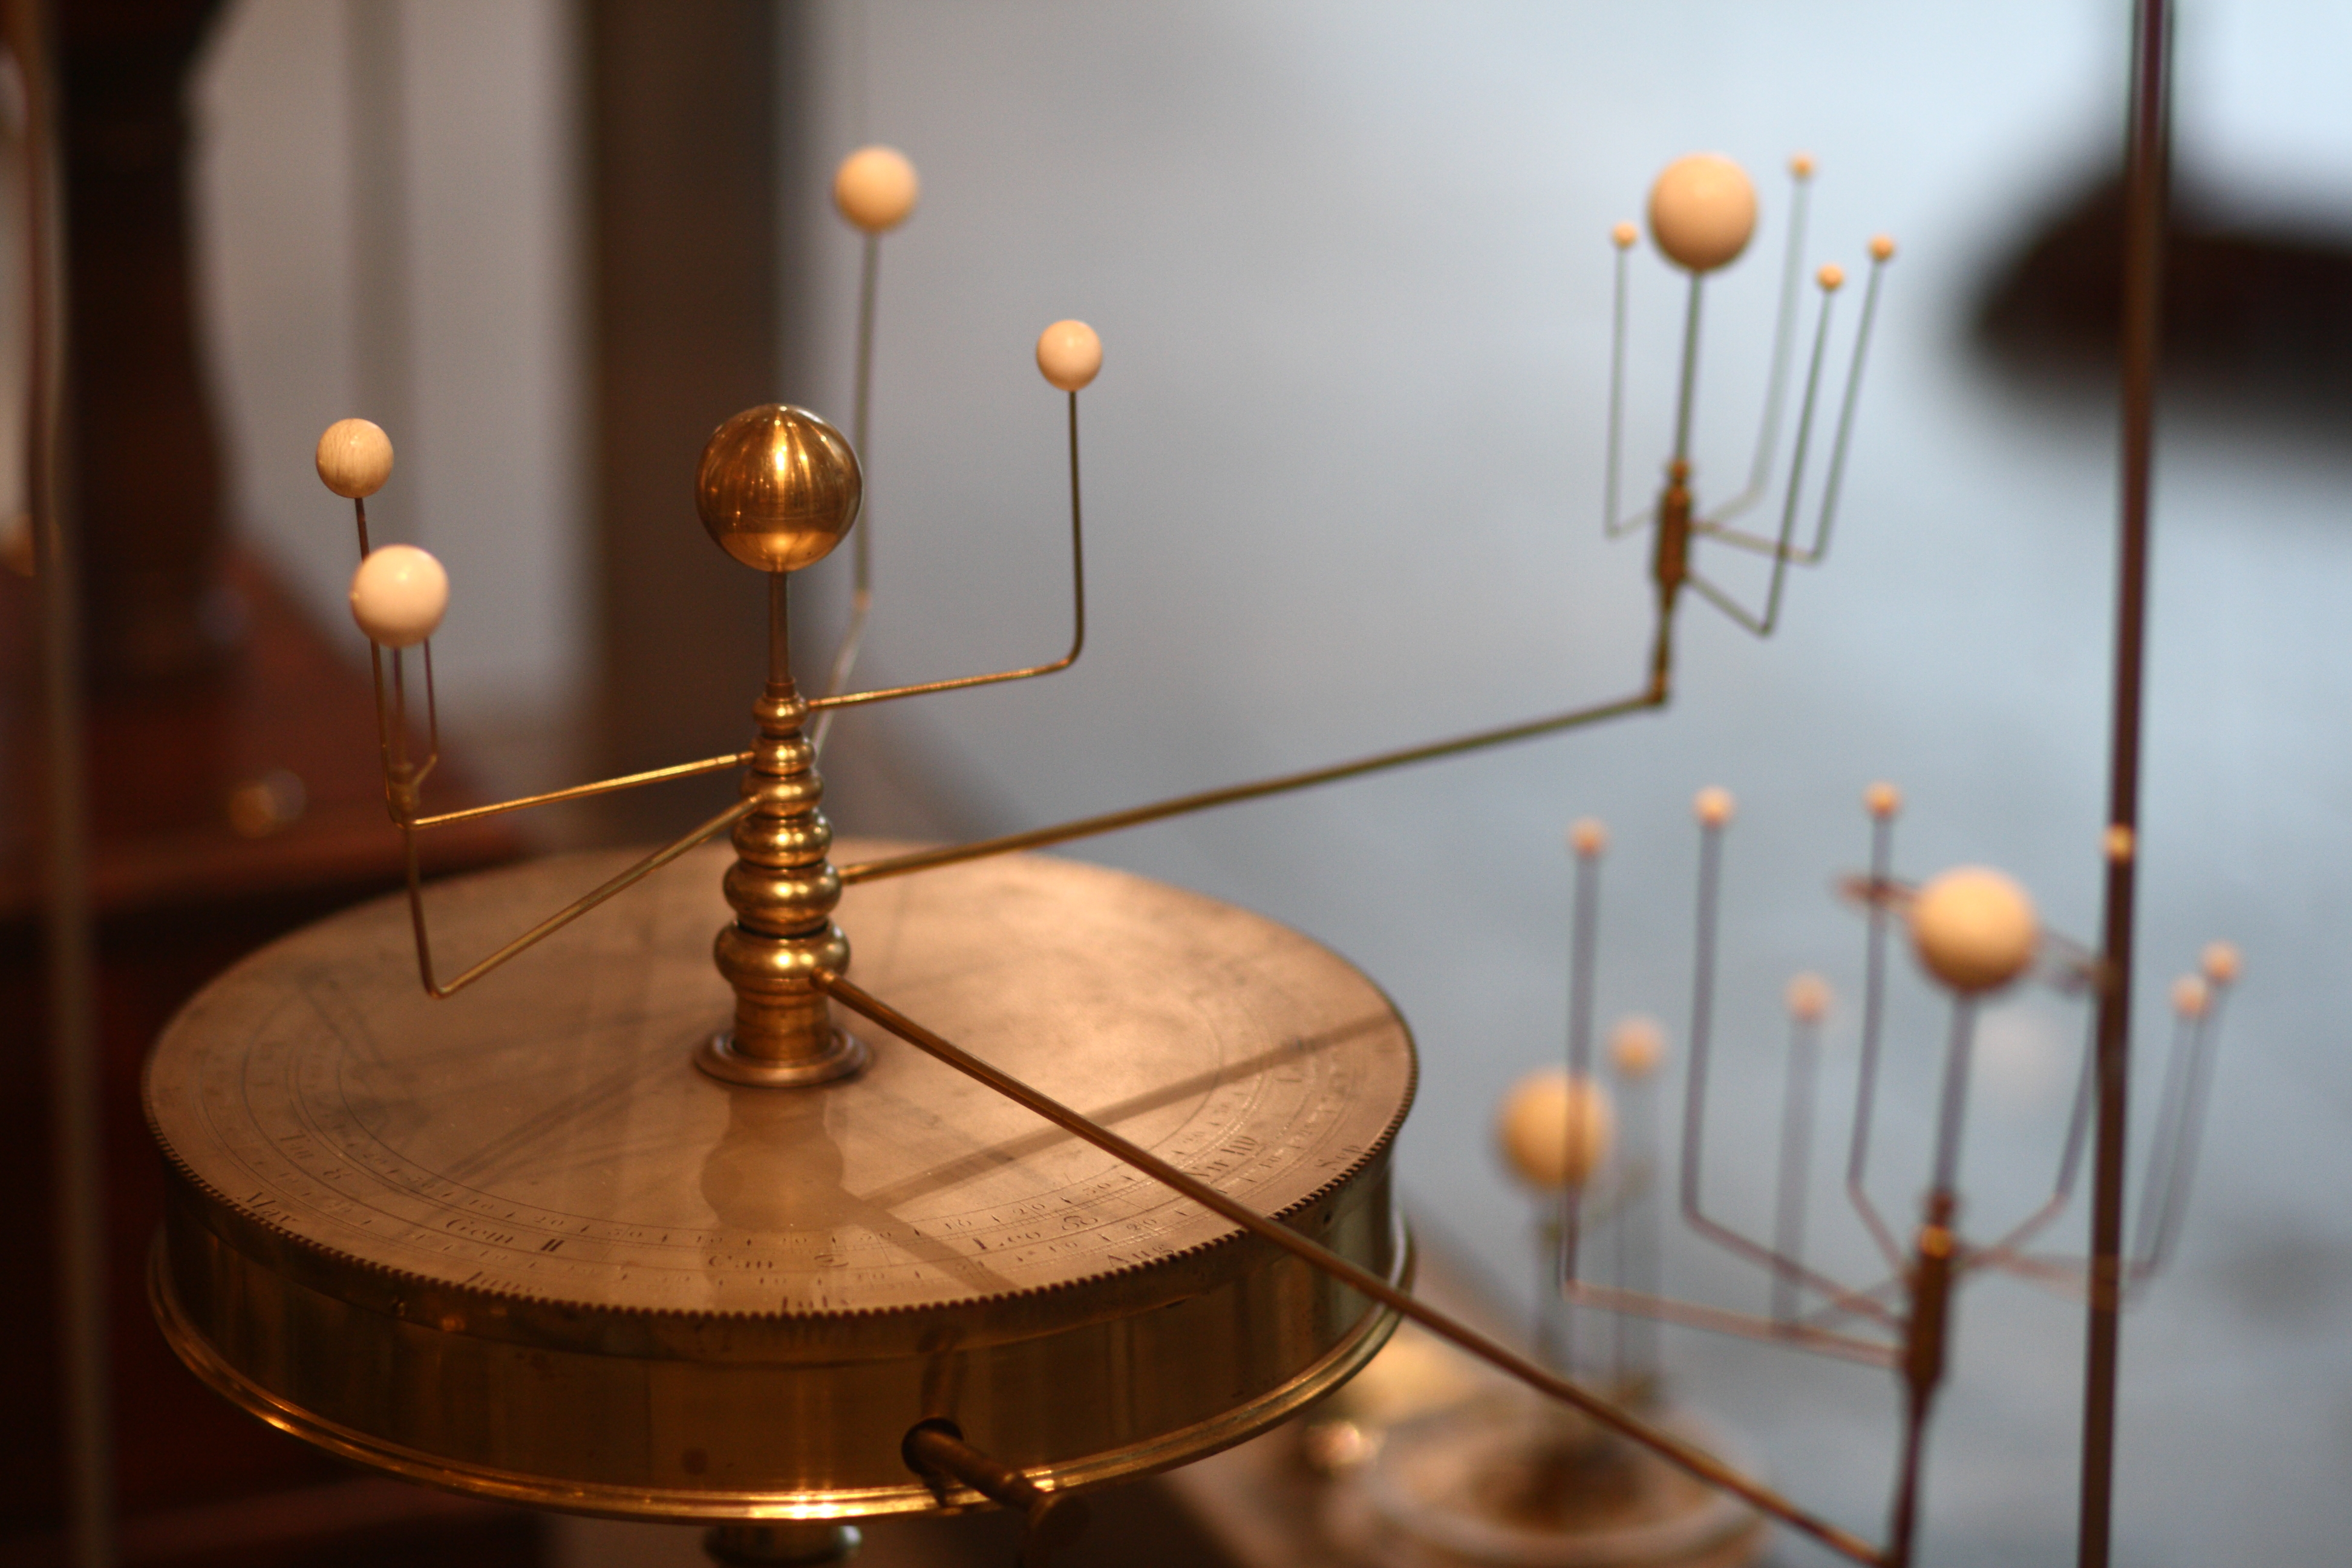
\includegraphics[width=0.45\textwidth]{images/SIM/orrery_Sage_Ross.jpg} \qquad \includegraphics[width=0.45\textwidth]{images/SIM/Baltic_Aviation_Academy_Airbus_B737_Full_Flight_Simulator_(FFS).jpg}
\caption[\small Harvard orrery; flight simulator]{\small Harvard orrery \cite{SIM_O}, and Baltic Aviation Academy Airbus B737 Full Flight Simulator (FFS) in Vilnius (public domain).}\label{fig:orr}\hrule
\end{figure}
\subsubsection{Types of Simulations}
We have already alluded to some types of simulations; in this section we provide more concrete descriptions of the avenues available to modelers. 
\paragraph{Full-Scale Physical Simulations}
Full-scale physical simulations are \textbf{life-sized}, \textbf{physically realistic} simulations, which  make use of structures that already exist to replicate or reproduce target system behaviours. \par For example, to simulate boat rescue situations (and then practice responding under various scenarios), the Coast Guard might make use of existing vessels and emergency personnel, and introduce actors playing the part of accident victims, a wave machine to simulate possible environmental conditions, etc. 

\paragraph{Mechanical Simulations}

A mechanical simulation is one that is physically implemented but which is not necessarily full-scale, to-scale or physically realistic in various other respects. It simulates dynamic behaviours using electro-mechanical components. Mechanical simulations were popular prior to the advent of computers. The `orrery', a classic type of clockwork model of the solar system, is a typical example of a mechanical simulation (see Figure~\ref{fig:orr}, left). Another example would be a CPR dummy that can be used to practice proper CPR technique, and which may have sensors to simulate certain heart behaviours and then provide feedback regarding the effectiveness of the applied CPR.

\paragraph{Computer (Programmatic) Simulations}

Programmatic simulations represent the target system or process using \textbf{data structures} and \textbf{algorithms}. The data structures are sets of variables that represent the properties of system objects, and the algorithms determine how these properties change over time. When quantitative consultants produce simulations, they are usually programmatic. 
\vfill
\begin{itemize}[noitemsep]
\item\textbf{Event-Centric Computer Simulations} -- This type of computer simulation models \textbf{activity} (and is dynamic in this sense), but the focus is not accurate modeling of time. The goal, rather, is to represent an event or sequence of events. For example, we might simulate the selection, and result, of sampling a population, or simulate possible outcomes of a series of events that themselves occur with particular probabilities.

\item \textbf{Discrete Time Computer Simulations} -- As suggested by the name, discrete time simulations treat time as a \textbf{discrete series of consecutive steps}, rather than continuously. A common example of this is the \textbf{agent-based} model (or multi-agent simulation); in this type of simulation, the time step may range from seconds to years, and the goal of the simulation is to explore how individual agents interact with each other over this time span.

\item \textbf{Continuous Time Computer Simulations} -- In contrast to discrete time simulations, continuous time simulations treat time as a continuous property. However, there is a challenge here, as continuous time simulations are generally implemented on a computer, and computers are necessarily discrete. Thus, in practice, a continuous time simulation is one where the discrete time steps are simply \textbf{very small}. Note  that this is not equivalent to implementing a continuous-time mathematical model on a computer and solving it using mathematical methods implemented as algorithms.
\end{itemize}
\paragraph{Hybrid Models}
It is also possible to create a model of a system where one part of the model is of one type and another part is of another type. A realistic flight simulator, for instance, might consist of a few full-scale physical components such as the cockpit, seats, etc. (possibly using part of an actual plane), while the experience of actually flying the plane is simulated via computer, and perhaps integrated with the physical part of the simulation by projecting a computer controlled image onto the cockpit window (see Figure~\ref{fig:orr}, right). The computer simulation might also controls the physical behaviour of the motion of the cockpit -- its pitch, yaw, and roll, for example.
\subsubsection{Strategies for Creating Models and Simulations}
Among practitioners, it sometimes said that modeling is as much an art as it is a science. While there are no tested and true approaches that will work no matter the situation under consideration, the following steps, illustrated in Figures~\ref{simfig:4} to \ref{simfig:9} with the simulation of a school of fish, often end up having practical importance in the process: 
\begin{itemize}[noitemsep]
\item gather information about the target system;
\item create a conceptual model; 
\item build the model; 
\item verify and validate, and
\item run and analyse. 
\end{itemize}
\paragraph{Gathering Information About the Target System}

As domain experts or modeling specialists, it can be tempting to believe that the understanding of the target system is so strong that that we can forgo collecting and validating information about that system and jump right into implementing a model of the system. However,  modelers tend to be experts in specific techniques rather than in the behaviour of the target system, and \textit{vice-versa} for the domain experts -- \textbf{teamwork} is usually required  to properly construct the model.
\newpage\noindent
In such a case, the modeler and domain expert must work together closely to \textbf{gather the information} about the system that the domain expert believes will be required to understand or predict the relevant behaviours of the target system. The modeler must also keep in mind the types of information required to create a comprehensive and consistent model of the system, given the proposed model type. Creating a \textbf{conceptual model} (see below) will greatly assist with the process of determining what information is necessary to properly \textbf{represent} the target system.
\newl There is also an opportunity to \textbf{validate} the structure of the model at this stage. Even when a domain expert is involved, ensuring that the information being incorporated into the model comes from \textbf{rigorous and reliable sources}, and \textbf{documenting these sources} early on, will enhance the likelihood that the model will be valid, as well as \textbf{increasing the credibility} of the model in the eyes of those using the model.
\begin{figure}[!t]
	\centering
		\includegraphics[width=0.45\textwidth]{images/SIM/Sixfinger_threadfin_school.jpg}
	\caption[\small A school of fish -- the target system for a fish school simulation]{\small A school of fish -- an example of a target system to be simulated \cite{SIM_FISH}.} 
	\label{simfig:4}\hrule
\end{figure}
\afterpage{\FloatBarrier}

\begin{figure}[!t]
	\centering
		\includegraphics[width=0.80\textwidth]{images/SIM/information_about_system2.pdf}
	\caption[\small Some information about fish perceptual mechanics]{\small Gathering information: relevant perceptual mechanics information about a single fish, to be incorporated into the model \cite{SIM_S}.}
	\label{simfig:5}
\end{figure}
\afterpage{\FloatBarrier}
\paragraph{Creating a Conceptual Model}

A \textbf{conceptual model} is a clearly defined description of those \textbf{components}, \textbf{properties}, and \textbf{relationships} of the system that are believed to be important, relative to the system behaviours or properties of interest (i.e. the \textbf{modeling context}). A conceptual model may be: 
\begin{itemize}[noitemsep]
\item a verbal description of the system, structured or organised in some way;
\item a collection of diagrams depicting elements of the system and their relationships, or 
\item a combination of both.
\end{itemize}
The conceptual model can be thought of as the \textbf{blueprint} that will be followed during construction of the model.

\begin{figure}[!t]
	\centering
		\includegraphics[width=0.70\textwidth]{images/SIM/conceptualmodel3schellinck2011.pdf}
	\caption[\small Representing the fish school in the simulation]{\small Creating a conceptual model: a conceptual model showing how elements of the target system -- the fish in a fish school -- will be represented in the model of the fish school \cite{SIM_S}.}
	\label{simfig:6}
\end{figure}
\afterpage{\FloatBarrier}

At this stage, the modeler will also often discover that it is necessary to define concretely the more abstract or less well defined elements of the target system, in preparation for implementing the model. As well, it may be determined during construction of the conceptual model that there are gaps in the understanding of the system itself, which prevent the construction of a complete model of the system. If this occurs, it may be necessary to return to gathering information about the target system itself. If the required information is not readily available it is important at this step to indicate which parts of the model are based on reliable knowledge about the system and which parts are speculative.
\newpage\noindent This step can be challenging from an interdisciplinary perspective because, as we have already mentioned, it requires the modeler and the domain expert to work together to create the conceptual model. For this step to proceed as it should, the domain expert must, in a sense, enter into the world of the modeler, just as the modeler must enter into the world of the domain expert. This can be difficult to achieve, for a variety of reasons, and as a result it can be tempting to to skip this step outright -- to leave the conceptual model in an implicit stage rather than an explicit stage -- and to jump straight into building the model. However, unless the modeler is a domain expert and the system itself is relatively simple, this can lead to models that do not perform satisfactorily when all is said and done.

\begin{figure}[!t]
	\centering
		\includegraphics[width=0.75\textwidth]{images/SIM/knowledge_to_model.pdf}
	\caption[\small Representing the physical characteristics of individual fish]{\small Creating a conceptual model: determining how specific relevant physical characteristics of individual fish will be represented and incorporated into the model \cite{SIM_S}.}
	\label{simfig:7}\hrule
\end{figure}


\paragraph{Building the Model}

Once the conceptual model is in place, a model type (e.g. mathematical, simulation) can be selected in order to \textbf{build the model} itself, using the conceptual model as a blueprint. Target system objects, properties and relationships are translated into model structures.

\begin{figure}[!t]
	\centering
		\includegraphics[width=0.85\textwidth]{images/SIM/implementation.pdf}
	\caption[\small Fish school simulation pseudo-code]{\small Building the model: pseudo-code describing how the simulation of the fish school is created \cite{SIM_S}.}
	\label{simfig:8}\hrule
\end{figure}

\begin{figure}[!t]
	\centering
		\includegraphics[width=0.9\textwidth]{images/SIM/simulatedfish3.png}
	\caption[\small A screen shot of the 3D fish school simulation]{\small Building the model: the resulting simulation of the fish school. The schooling behaviour is an emergent property of the simulation, coming out of programmed individual simulated-fish behaviours \cite{SIM_S}.}
	\label{simfig:9}\hrule
\end{figure}

\paragraph{Verifying and Validating}

Verifying the model means going over the model in order to confirm that it has been \textbf{constructed as intended}, given the conceptual blueprint that has been developed. Validation refers to a process of confirming that the constructed model is in fact a \textbf{good match} for the target system. Thus, a model could be verified as having been constructed as intended, but the model might still be invalid if, for example, the modeler was misinformed about the actual workings of the target system. A thoughtful discussion of model validation, in the context of building population-based disease simulation models, can be found in \cite{SIM_KFMBF}.

\paragraph{Running and Analysing}

Once the model has been verified and validated, it may then be analysed in order to \textbf{draw conclusions} about the target system. In the case of simulations, model parameters have to be selected, and `runs' of the model carried out for each set of parameters. A `run' here means that the model is given certain initial starting conditions and then the behaviour of the simulation allowed to proceed and produce various outputs of interest. If the model has stochastic components, it may be necessary to carry out multiple runs using the same parameter settings in order to produce posterior distributions for the outputs. Once the simulation has been run with all of the relevant parameter settings, the resulting output of the simulation can be analysed. At this point, the analysis may follow any of a vast number of methods: trend extraction and forecasting, classification, data visualisation, etc. 


\subsubsection{Computational Complexity of Simulations}

Because simulations are computer programs, it remains crucial  to be aware of the broader issue of \textbf{computational complexity} when constructing simulations. The computational complexity of an algorithm is based on the number of possible steps in the algorithm and how they interact with different types of data to lead to different run times. \par Although a detailed discussion of computational complexity is beyond the scope of this section, understanding that the manner in which the simulation is programmed will influence its run time is very important, as this  might limit the options for the exploration of parameter space.\newpage\noindent
As previously discussed, when a simulation is created, a set of parameters to vary has to be explicitly selected in order to explore the behaviour of the simulation. However, because specific parameter values have to be chosen for each run of the simulation, and because multiple simulations have to be run in order to get a general sense of the behaviour of the simulation (i.e. building a posterior distribution for the behaviour), and by extension the system, the problem of \textbf{combinatorial explosion} is encountered  very quickly. The problem cannot always be bypassed, and it might be that the best that can be hoped for is to maximise the number of simulation runs that the computer can support in the available time.

\begin{figure}[!t]
	\centering
		\includegraphics[width=\textwidth]{images/SIM/program_complexity.png}
	\caption[\small A sketch of computational complexity]{\small A sketch of some different possible computational complexities of a computer program, as represented in Big-O notation.}
	\label{simfig:10}\hrule
\end{figure}
\afterpage{\FloatBarrier}
\subsubsection{Model and Simulation Applications}

\paragraph{Science} The appropriate role of models and simulations within science is a topic for debate within scientific circles. Statistical models are well accepted and used extensively. Mathematical models are generally accepted if used in a theoretical context. In our experience, however, the use of simulations is currently not well tolerated. In situations where carrying out actual experiments would be difficult (e.g. for ethical reasons), simulations may be viewed as a type of virtual experiment. In such situations the results of the virtual experiment, although not viewed in the same light as actual experimental results, may, at the very least, usefully fuel the discovery of hypotheses, which may then be tested using other methods.


\paragraph{Business} Accurate prediction of events is highly valued in a business context. As a result the emphasis for models in this domain is on predictive accuracy, rather than on being able to use the model for explanatory purposes. Businesses use models to, for example, predict customer behaviour, how their business will be affected in certain market situations, and how they might reorganise their business structure to reduce overhead and increase profitability.

\paragraph{Government} A major activity within the government is setting policy. Within this context, it is often important to explore different possible policy scenarios, and gain a better understanding of which policies will be more or less effective under a variety of circumstances. Models that provide explanatory power can be particularly helpful in this type of work, because it allows for an understanding of why one approach might work better than another. This can then be taken into account in order to ensure good policy.

In addition, as with businesses, the government is interested in making its own operations more efficient and effective. From an organisational perspective models can be useful in determining the best strategies for internal structures and processes, as well as the conditions under which such structures may function more or less optimally.
\vfill\newpage\noindent
\paragraph{Education} Simulations play an important role in education. They allow students to explore and experience scenarios in a virtual manner, which both decreases the potential consequences of learning through doing, and increases the possibility to learn from experiences in controlled and monitored conditions. For a very thorough discussion of the role of simulations in education, see \cite{SIM_L}.


\paragraph{Entertainment} It might be argued that most forms of entertainment are simply reflections or representations of real world experiences, and thus are, in some sense, models of life, broadly speaking. More specifically, simulations and models frequently play an important role in theatre, television and film -- allowing the creators of such media to convincingly mimic real life situations without needing to entirely re-create or enact them. Use may be made of physical small-scale models (e.g. a small-scale model of a cityscape), life-size models of particular environments (e.g a life-size model of a submarine) or computer simulations (e.g. simulated flocks of birds and artificially generated clouds, added to give more realism and detail to the backdrop of a scene).

\subsubsection{Modeling and Simulation Software}

It is quite possible to create models by hand, without the use of computers, and it is also possible to create computer models or simulations without using a particular programming environment. Some programming environments have been specifically designed for creating simulations. Some of these currently available (as of 2018) include:

\begin{itemize}[noitemsep]
    \item Matlab Simulink (commercial simulation software)
    \item Simio (commercial simulation software)
    \item Netlogo (free software, mainly for teaching and prototyping)
    \item SymPy (a python library for discrete time simulations)
\end{itemize}

\subsubsection{Case Study: NWMO}
Canada has a long history with nuclear power: the first self-sustained Canadian nuclear reaction was achieved at Chalk River's ZEEP reactor in 1945. Over the years, numerous research reactors and power reactors have been built and decommissioned -- as of 2014, electricity is currently being produced by 19 CANDU reactors in Ontario and New Brunswick. Given that the existence of high energy nuclear waste in Canada is a \emph{fait accompli} -- we have already chosen, as a society, to use nuclear power and create nuclear waste --  it is paramount that we find ways to safely dispose of this waste. 
\par
In 2002, the \textit{Nuclear Fuel Waste Act} (NFWA) was enacted to study possible strategies for the management of Canada's used nuclear fuel. As a result, the \textit{Nuclear Waste Management Organization} (NWMO) was formed by the Canadian nuclear power companies, with the mandate to provide recommendations to the Canadian Government for the long-term management of used nuclear fuel. One such recommendation, which was accepted in 2007, was the establishment of Adaptive Phased Management (APM) as both a social and technical approach to permanently manage Canada's used nuclear fuel. Canadian citizens determined that the optimal strategy, given the current state of technology in Canada, is the construction of a deep geological repository to contain and isolate the fuel.
\newl
This decision puts the NWMO in a unique and demanding position, as it is the first group in Canada to design and build a unique but extremely performance-critical engineering structure: a long term Canadian repository for high energy nuclear waste. By its very nature, this structure as a whole cannot be tested in advance of use and essentially cannot be maintained once it is built. Furthermore, the environment and materials involved are themselves volatile and their long term behaviour is difficult to predict.
\par
Under such challenging circumstances, engineers must do their best to use all of the expertise at their disposal to create as perfect a design as possible for the required structure. Despite the uniqueness of the structure, they need to produce a design that will meet the requirements that have been set out, and then, once built, function exactly as predicted on the first try.  Such a design process is necessarily a lengthy one, involving many designers with high levels of expertise. Many designs would be proposed and rejected before a final design is selected, based on all the evidence and expertise the design team have at their disposal.
\par
At the end of the process the engineering team will have high confidence in the final design that is put forward. The success of the structure in question is critical, and, as responsible, professional engineers, they would not put forward a design for such a structure without being entirely certain, to the best of their collective ability, that this structure will not fail.
\par
Despite this confidence, due diligence requires more than the simple assurance (and belief) from the design team that the structure will not fail. It is not enough, from a societal perspective, for the team to simply provide a ``vote of confidence:'' it also requires the provision of more quantitative information about the failure aspects of the structure. Those responsible for the structure need to be able to determine (and to help the stakeholders understand) what are the structure's necessary and sufficient conditions for failure (and by extension, the conditions for non-failure). To produce these answers they need to be able to quantitatively examine what circumstances the structure might encounter, and under these circumstances, what the probability of failure is.
\newl
From an ideal testing point of view, the entire proposed structure would be built many times over to run trials relating to each of the foreseen circumstances. Data would then be gathered and analyzed to determine the failure tolerance of the structure. Failure probabilities would be calculated based on this data, along with an understanding of possible failure circumstances -- the structure might even be redesigned to take into account the results of the testing. 
\par
However, as we have already noted, this idealistic testing scenario is simply not an option in this case. The structure as a whole cannot be directly tested even once, let alone multiple times. And on top of this, even were many replications of the structure itself available for testing, not all failure circumstances (in particular those involving major geological forces and long time spans) would be possible to re-create in a test environment.
\newl
An alternative strategy is centered around a combination of physical testing and modeling of the behaviour of the structure and environment. More specifically, a larger structure is built up of many component parts, which themselves may be built up of many components. The failure parameters of these component parts may be tested, even if the structure as a whole cannot. \par Similarly, while the structure itself, and perhaps even in some cases the components themselves, cannot be tested repeatedly, there remains the option of creating models of the structure and components in question, and then using the behaviour of these models to predict the behaviour of the components and, in turn, of the structure at large.
\newpage\noindent
In the absence of the ideal testing scenario, understanding and quantifying the failure of the system as a whole can be carried out by understanding and quantifying the failure circumstances of the components of the system, understanding the causal relationships between these components, creating models of the system as a whole based on these relationships, determining the failure circumstances and probabilities of the constructed structure level models and then transferring these findings over to the structure itself. This results in an estimate of the failure circumstances and probabilities of the actual engineered structure as a whole.
\newl
The end result of this exercise will thus be, rather than a simple yes/no statement (such as ``No, the structure will not fail'', for instance), a list of the possible failure circumstances and an estimate of the failure probabilities for both the structure components and the structure itself, along with a confidence measure indicating a level of confidence in the failure probabilities calculated for each failure circumstance.
\par Such a table of failure circumstances, probabilities, and confidence measures will allow those building the structure to open a legitimate dialogue with those responsible for, and those being affected by, the resulting structure. In essence, this deliverable will allow the designers of the structure to provide their stakeholders with a clearer and more detailed picture of the risks they are likely to encounter when undertaking the construction of such a structure.
\paragraph{General Objectives}
The general objective of this Failure Analysis project as a whole is to estimate the failure probability of the Mark II canister and engineered barrier system immediately surrounding the canister. In order to achieve that larger objective, we anticipate that we will be using a combination of statistical analysis, mathematical modeling, and simulations, much as in this prototype. More specifically, we will take the approach that our model is meant to answer a specific question, as well as to provide outputs that can be fed into other models, as may be required by already-developed NWMO models.
\par In this prototype phase, however, the objective is to develop a methodology and implementation framework to confirm that interactions (both planned and emergent) can in principle be captured by the modeling process, both at the repository and the manufacturing level. For both the manufacturing process and the interactions models, a  specific selection of a small number of sub-components of the entire system will be considered in this phase, in order to maintain focus on the development and testability of the methodology itself.  
\begin{center}\rule{0.5\linewidth}{.4pt}\end{center}
In the following extract from the report Failure Analysis Simulation Model for the APMRD-II, we discuss some of the strategies that could be used to extract information and knowledge about the engineered barrier system, which could then be incorporated in any interaction model of its components. A discussion of system complexity and the effect it had on our choice of modeling approach is also provided. We also provide a prototype UFC manufacturing process model: potential states, actions and variables are introduced, as well as the underlying modeling assumptions and families of parameters. The model is illustrated \textit{via} a specific parameter set; a series of 8 scenarios showcase the effect of various parameter combinations. \par \textbf{It should be noted that due to the uncertainty relating the manufacturing process parameters, the numbers presented in this section mostly play the roles of placeholders: reasonable estimates for a large number of these parameters will be required before the model can output meaningful failure estimates.}     

\phantomsection
\begin{thebibliography}{99}
\bibitem{SIM_C} Clement, J.J. [2008], Creative Model Construction in Scientists and Students: The Role of Imagery, Analogy, and Mental Simulation, Springer Netherlands, 10.1007/978-1-4020-6712-9
\bibitem{SIM_HGK} Holyoak, K., Gentner, D., and Kokinov, B. [1998], Introduction: The place of analogy in cognition, In Holyoak, K., Gentner, D., and Kokinov, B. (eds.), Advances in Analogy Research: Integration of Theory and Data from the Cognitive, Computational, and Neural Sciences, NBU Press, Sofia.
\bibitem{SIM_H} Hofstadter, D.R. [2001], Analogy as the core of cognition, In Gentner, D., Holyoak, K., and Kokinov, B., (eds.), The Analogical Mind: Perspectives from Cognitive Science, The MIT Press Bradford Book, Cambridge MA.
\bibitem{SIM_KFMBF} Kopec, J.A., Fin\`es, P., Manuel, D., Buckeridge, D., Flanagan, W.M., Oderkirk, J., Abrahamowicz, M., Harper, S., Sharif, B., Okhmatovskaia, A., Sayre, E.C., Rahman, M.M., and Wolfson, M. [2010], Validation of population-based disease simulation models: A review of concepts and methods, BMC Public Health, 10. 10.1186/1471-2458-10-710.
\bibitem{SIM_L} Landriscina, F. [2013], Simulation and Learning: A Model-Centered Approach, New York, NY: Springer, 10.1007/978-1-4614-1954-9. 
\bibitem{SIM_S} Schellinck, J. [2009]. A general perception based framework for modelling animal aggregation, Carleton University, Ottawa.
\bibitem{SIM_Y} Yilmaz, L. (ed.) [2015], Concepts and Methodologies for Modeling and Simulation: A Tribute to Tuncer \"Oren, Springer International Publishing, Switzerland, 10.1007/978-3-319-15096-3.
\bibitem{SIM_P} Pearl, J. [2009], Causality: Models, Reasoning, and Inference (2nd ed.), Cambridge University Press.  
\bibitem{SIM_T} Templ, M. [2016], Simulation for Data Science with R, Packt Publishing. 
\bibitem{SIM_TSAM} Attribution: By Fourdee (talk) (Uploads) - Own work, Public Domain, \newhref{https://en.wikipedia.org/w/index.php?curid=8650757}{https://en.wikipedia.org/w/index.php?curid=8650757}
\bibitem{SIM_NBP} \newhref{https://en.wikipedia.org/wiki/N-body\_problem}{https://en.wikipedia.org/wiki/N-body\_problem}
\bibitem{SIM_B} Beloriszky, D. [1930], Application pratique des m\'ethodes de M. Sundman \`a un cas particulier du probl\`eme des trois corps, Bulletin Astronomique 6 (series 2), 417–434.
\bibitem{SIM_LC} Cixin, L. [2008], The Three Body Problem, Chongqing Press.
\bibitem{SIM_WUM} \newhref{http://weusemath.org/?didyouknow=new-discoveries/n-body-problem}{http://weusemath.org/?didyouknow=new-discoveries/n-body-problem}
\bibitem{SIM_NBODY} \newhref{https://en.wikipedia.org/wiki/N-body\_simulation}{https://en.wikipedia.org/wiki/N-body\_simulation}
\bibitem{SIM_NBODY1} Momkov, T. [2013], Planetary System Formation 2, $N-$body simulation, \newhref{http://trekto.info/n-body-simulation}{http://trekto.info/n-body-simulation}
\bibitem{SIM_O} Ross, S. [2009], A 1766 Benjamin Martin Orrery, used at Harvard (photo), \newhref{https://upload.wikimedia.org/wikipedia/commons/b/bf/Planetarium\_in\_Putnam\_Gallery_2\%2C\_2009-11-24.jpg}{https://upload.wikimedia.org/wikipedia/commons/b/bf/Planetarium\_in\_Putnam\_Gallery\_2\%2C\_2009-11-24.jpg}
\bibitem{SIM_FISH} \newhref{https://en.wikipedia.org/wiki/Shoaling\_and\_schooling}{https://en.wikipedia.org/wiki/Shoaling\_and\_schooling}
\end{thebibliography}

\setboolean{@twoside}{false}
\includepdf[pages={2},offset={50 -40}]{documents/ES_TC_NWMO.pdf}
\includepdf[pages={13-62},offset={50 -40}]{documents/ES_TC_NWMO.pdf}
\setboolean{@twoside}{true}




